\chapter{进程管理}
\section{进程生命周期和资源复用}
\subsection{进程生命周期}
进程指的是在系统中运行的一个程序的实例。而进程的生命周期包括从创建,就绪,阻塞,运行中,退出。
\begin{figure}[htb]
    \centering
    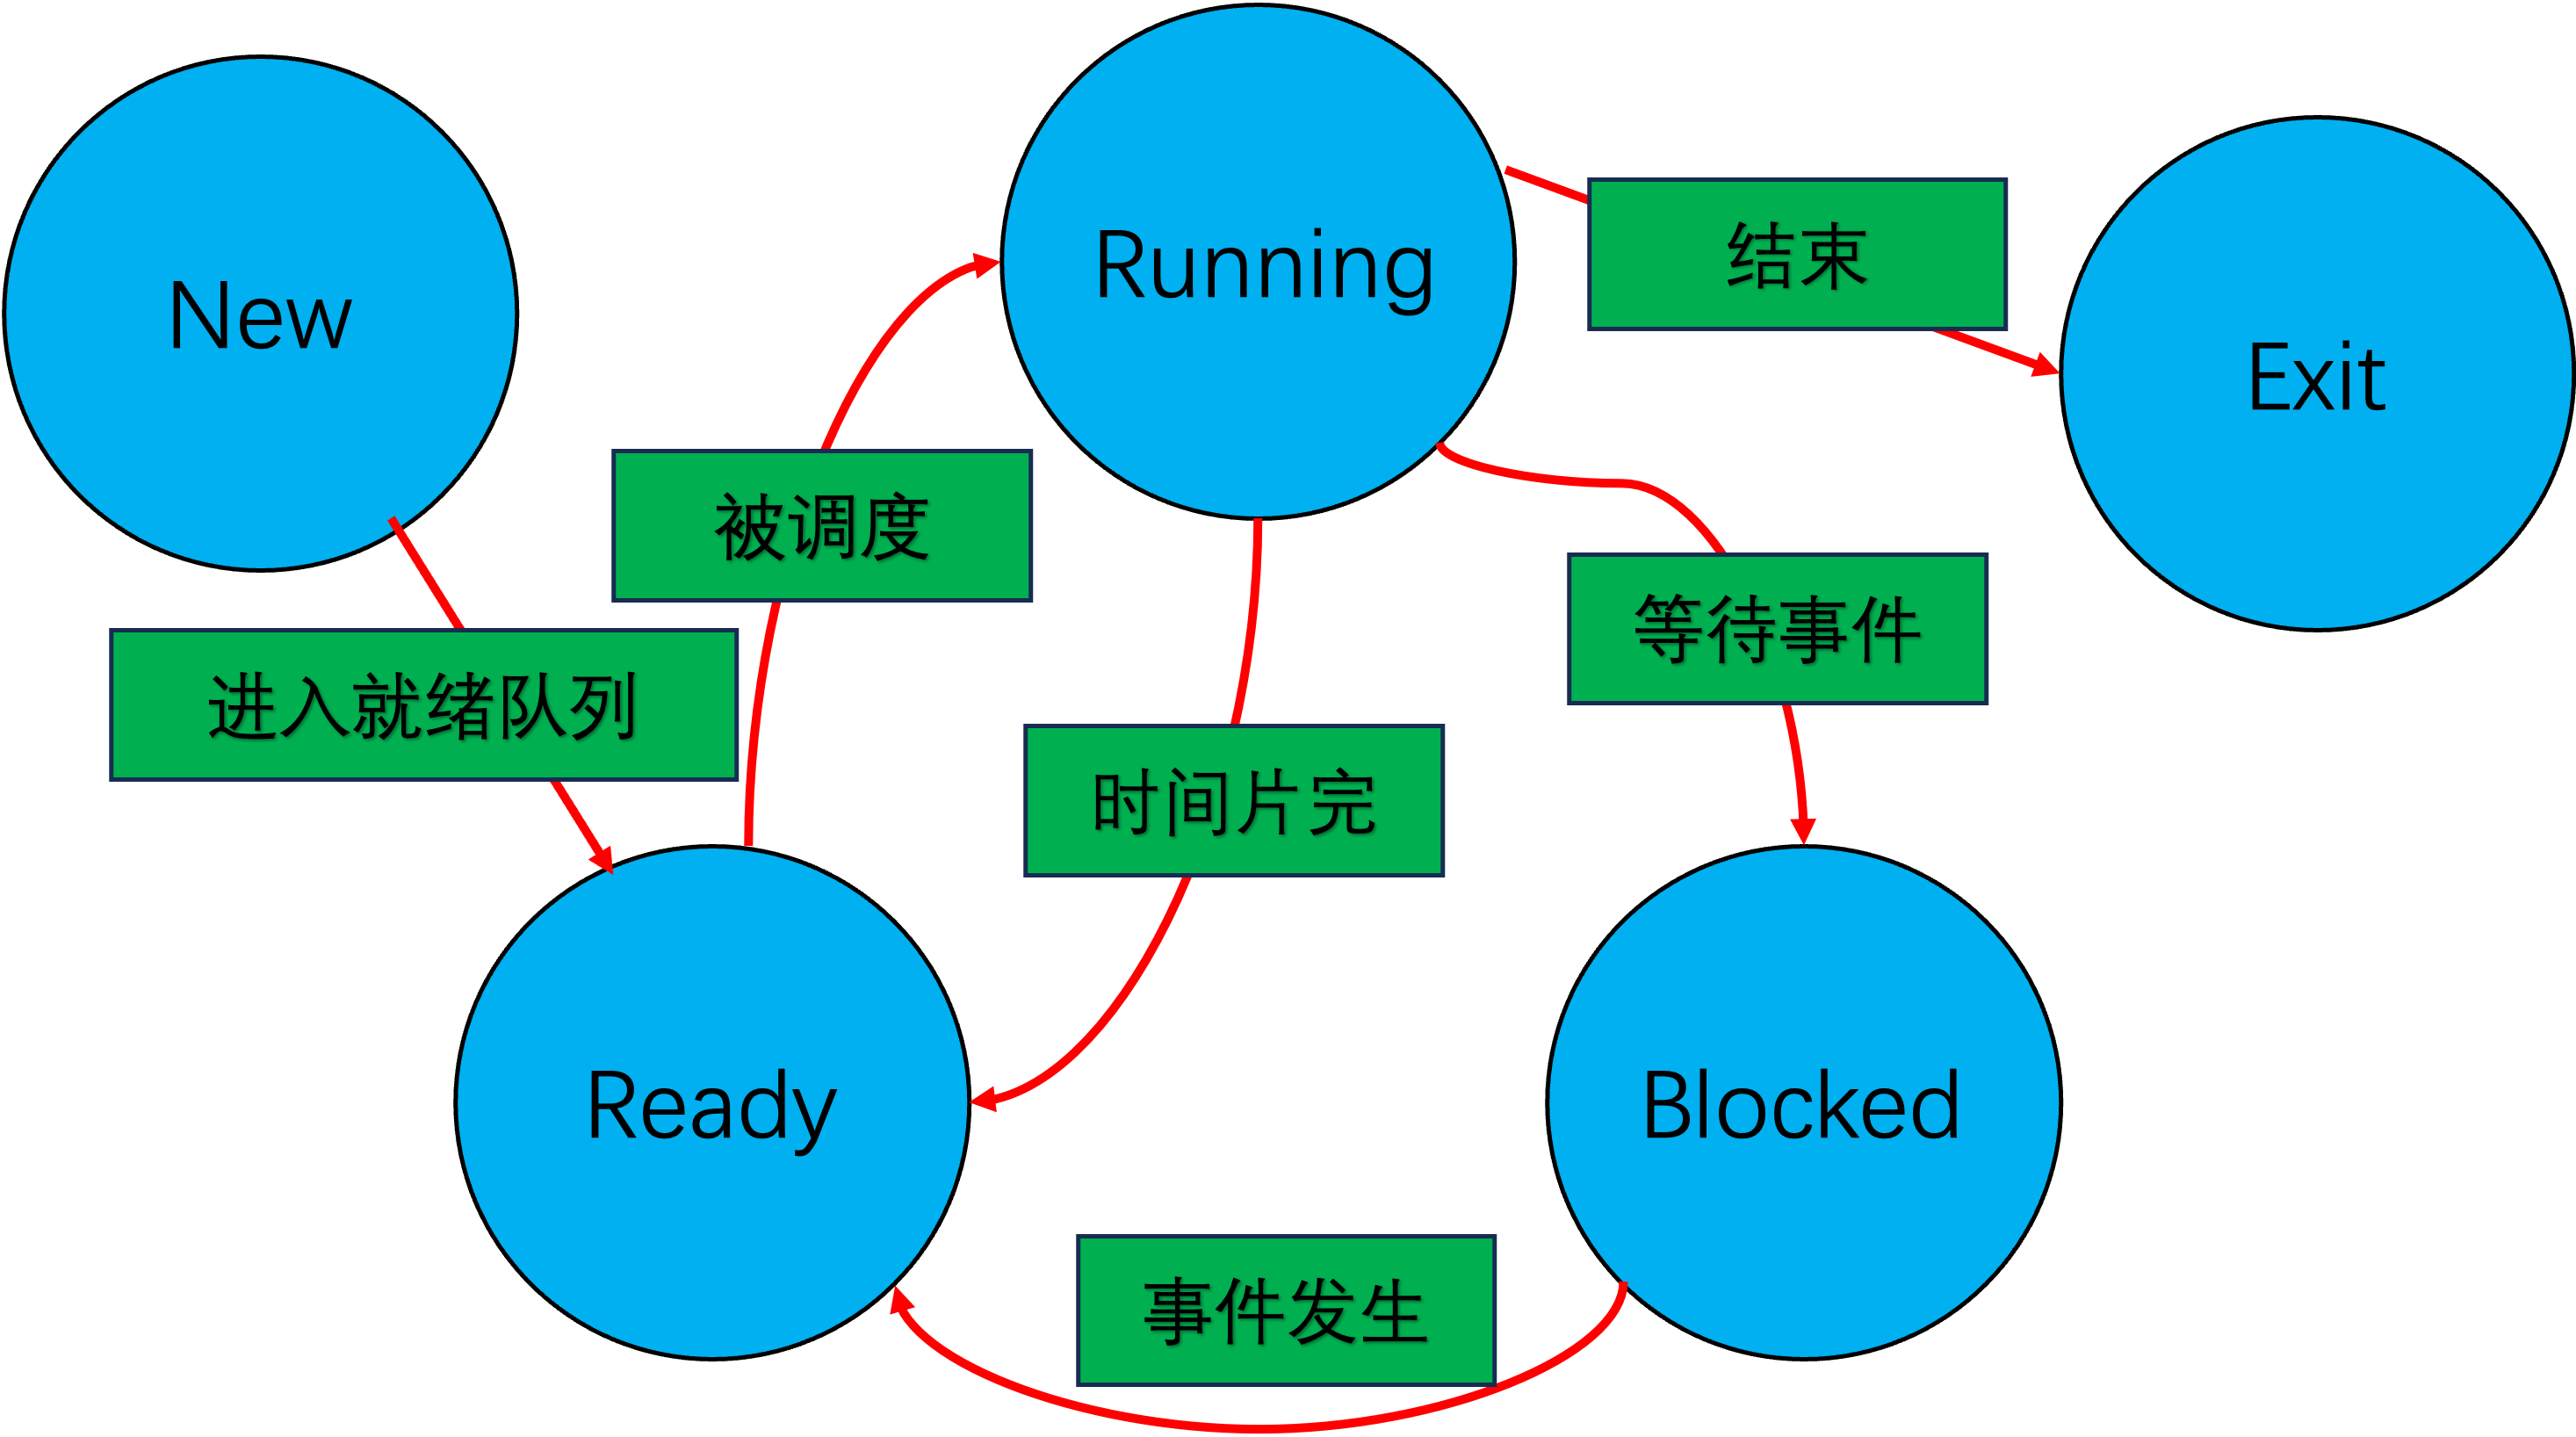
\includegraphics[width=\textwidth]{figures/05-01-进程生命周期示意图.png}
    \caption{
        进程生命周期示意图
    }
    \label{fig:user virtual process}
\end{figure}
在一个进程被创建之后,他会进入npucore中的就绪队列,在被操作系统调度之后将会进入到运行状态。
在运行状态下时间片耗尽或者是主动让出CPU的时候,进程会进入到就绪队列中,等待下一次被调度。
在运行的时候调用诸如wait等系统调用,进程会进入到阻塞队列中,等待被唤醒。
当进程执行结束,他会退出,释放系统资源。
npucore团队在进行性能调优之时,发现在操作系统运行示例程序时,IO操作导致CPU挂起的性能损失非常之大,因此我们将调度器进行了大改,使其完全支持了阻塞式的进程调度模式。
阻塞和非阻塞IO是访问设备的两种模式,驱动程序可以灵活的支持者两种用户空间对设备的访问方式。
阻塞操作是指在执行设备操作时,若不能获得资源,则挂起进程直到满足可操作的条件后再进行操
作。被挂起的进程进入睡眠状态,被调度器的运行队列移走,直到等待的条件被满足。
非阻塞是指在不能进行设备操作时,并不挂起,他要么放弃,要么不停地查询,直到可以进行操作为止。
在阻塞访问时,不能获取资源的进程将进入休眠,它将会让出CPU,因为阻塞的进程会进入休眠状态,所
以必须要有一个动作能唤醒该进程,唤醒进程的地方最大的可能发生在中断里面,因为在硬件资源获得的
同时往往伴随着一个中断。而非阻塞的进程则不断的尝试,直到可以进行IO。
与 linux 操作系统的设计类似, npucore采用等待队列的方式实现阻塞式调度器,将在后续章节介绍。
为了可以在npucore上同时运行多个进程,npucore实现了进程的创建,在内核中加载进程到内存,同时为其分配系统资源。
npucore为每一个进程分配系统资源,包括内存、文件描述符、CPU等,而实现系统资源的分配的方式是通过系统调用fork。
npucore中,fork系统调用用于创建一个新的进程,新的进程称为子进程,原来的进程称为父进程。
而所有的其他进程都是initproc的子进程,他们通过fork得到。initproc是需要在内核启动过程中创建的第一个进程。
对应的代码如下:
\begin{lstlisting}[language=rust]
    lazy_static! {
    pub static ref INITPROC: Arc<TaskControlBlock> = Arc::new({
        let elf = ROOT_FD.open("initproc", OpenFlags::O_RDONLY, true).unwrap();
        TaskControlBlock::new(elf)
    });
}
\end{lstlisting}
当创建一个新的进程时,用户进程通过fork得到一个原本进程的副本,为其分配系统资源,然后调用execve来讲elf文件加载到内存以创建一个新的进程。
每个进程都有自己的内存空间、代码和数据,它们是系统中资源的分配单位。他们的创建是由elf文件指定的。

为了保证所有的进程都能够被调度,从而避免进程饥饿的发生,npucore实现了进程的调度机制,从而实现阻塞和唤醒。
当一个进程主动放弃CPU或者被动的被剥夺CPU的使用权时,它会让出CPU,变成等待状态,这个过程称为阻塞。
在进程的视角看来,他会有一个自己独占CPU的“幻觉”,因为每一个阻塞和唤醒的时候进程的状态总是保持不变的。这样可以保证进程执行的正确性。
而npucore让一个被阻塞的进程重新开始执行的行为叫做唤醒。唤醒的同时会恢复进程的现场,包括阻塞时的寄存器状态。

而当一个进程执行结束,它就会退出,将它所占有的系统资源释放。进程的退出保证了npucore避免出现资源的永久占用的情况。
上述过程就是一个进程从“生”到“死”,保证了npucore可以正确且高效的执行对应的程序。

\subsection{资源复用}
为了实现多进程同时运行,操作系统需要对CPU,内存,外设等资源进行复用。
复用在资源有限的情况下是一个常用且实际的思想。围绕着复用的思想,我们可以提出以下几个问题:

如何实现上下文切换?

虽然保存现场思想是简单的,但是实际的实现却不是那么显然。在npucore中我们使用了一段所有进程共享的跳板代码和一个进程的私有的保存现场的帧来实现。

如何让进程如何实现透明调度,也就是用户进程不知道自己被调度了?

npucore实现了内置的计时器,当计时器中断发生时,内核会调用schedule函数,从而实现进程的调度。

进程的资源回收不能由进程自己来完成,否则进程退出时会出现资源泄露的情况,如何实现进程的资源回收?

npucore在exit之后,会释放一部分资源,但是不会释放所有的资源,从而进入僵尸状态,父进程来完成剩下的进程资源的回收。

如何在并发的情况下不会错过对进程的唤醒?

npucore中是一个单核的操作系统,在进入关键代码的时候会保证CPU不会调度其他进程,从而保证了进程的唤醒不会被错过。

此外,在内存方面,npucore采用了虚拟内存的方式,将物理内存映射到虚拟内存,从而实现了内存的复用。
对于用户的elf程序,程序的入口总是相同的,从某种程度上讲,程序将会“共享”同一个地址。
但是实际上,物理地址并不能被共享,所以虚拟内存就派上了用场。在上一章我们已经介绍了虚拟内存的实现,这里不再赘述。
I/O设备的复用将在I/O章节详细介绍。在这一章中,我们将介绍进程所拥有的各种内核的资源,诸如文件描述符等。

管理进程时,npucore使用了TCB的数据结构,不同于传统的PCB数据结构,npucore将线程视为共享栈的进程。
TCB的数据结构如下:
\begin{lstlisting}[language=rust]
pub struct TaskControlBlock {
    // immutable
    pub pid: PidHandle,
    pub tid: usize,
    pub tgid: usize,
    pub kstack: KernelStack,
    pub ustack_base: usize,
    pub exit_signal: Signals,
    // mutable
    inner: Mutex<TaskControlBlockInner>,
    // shareable and mutable
    pub exe: Arc<Mutex<FileDescriptor>>,
    pub tid_allocator: Arc<Mutex<RecycleAllocator>>,
    pub files: Arc<Mutex<FdTable>>,
    pub fs: Arc<Mutex<FsStatus>>,
    pub vm: Arc<Mutex<MemorySet>>,
    pub sighand: Arc<Mutex<Vec<Option<Box<SigAction>>>>>,
    pub futex: Arc<Mutex<Futex>>,
}
\end{lstlisting}
在上面的定义中,我们可以看到TCB中包含了进程的进程号,线程号,线程组号,内核栈,用户栈,退出信号,以及一些共享的资源。
后面将具体讲解如何管理这些资源以及进程之间的调度。